\documentclass[tikz]{standalone}
\usepackage{fontspec}
\setmainfont{STSong} % 设置文档的主要字体为宋体

\usetikzlibrary{angles, quotes}

\begin{document}
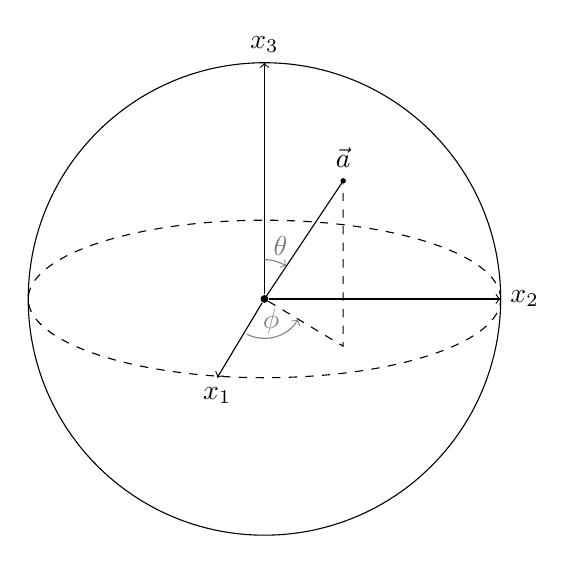
\begin{tikzpicture}

  % 定义 Bloch 矢量的模长
  \def\r{3}

  % Bloch 矢量
  \draw (0, 0) node[circle, fill, inner sep=1] (orig) {} -- (\r/3, \r/2) node[circle, fill, inner sep=0.7, label=above:$\vec{a}$] (a) {};
  \draw[dashed] (orig) -- (\r/3, -\r/5) node (phi) {} -- (a);

  % 画 Bloch 球
  \draw (orig) circle (\r);
  \draw[dashed] (orig) ellipse (\r{} and \r/3);

  % 坐标轴
  \draw[->] (orig) -- ++(-\r/5, -\r/3) node[below] (x1) {$x_1$};
  \draw[->] (orig) -- ++(\r, 0) node[right] (x2) {$x_2$};
  \draw[->] (orig) -- ++(0, \r) node[above] (x3) {$x_3$};

  % 角度
  \pic [draw=gray, text=gray, ->, "$\phi$"] {angle = x1--orig--phi};
  \pic [draw=gray, text=gray, <-, "$\theta$", angle eccentricity=1.4] {angle = a--orig--x3};

\end{tikzpicture}
\end{document}
